\documentclass[12pt]{article}
\author{Lawrence Liu}
\usepackage{subcaption}
\usepackage{graphicx}
\usepackage{amsmath}
\usepackage{pdfpages}
\newcommand{\Laplace}{\mathscr{L}}
\setlength{\parskip}{\baselineskip}%
\setlength{\parindent}{0pt}%
\usepackage{xcolor}
\usepackage{listings}
%\definecolor{backcolour}{rgb}{0.95,0.95,0.92}
\usepackage{amssymb}
\usepackage[T1]{fontenc}
\usepackage{beramono}%\lstdefinestyle{mystyle}{
%    backgroundcolor=\color{backcolour}}
%\lstset{style=mystyle}
%\usepackage[usenames,dvipsnames]{xcolor}%%
%% Julia definition (c) 2014 Jubobs
%%



\title{ECE 133A HW 4}
\begin{document}
\maketitle
\section*{Exercise A5.6}
\subsection*{(a)}
Let $DX+XD=A$, we have that $A_{ij}=(D_{ii}+D_{jj})X_{ij}$,
Since $DX+XD=B$ we have that 
$$A_{ij}=B_{ij}$$
$$B_{ij}=(D_{ii}+D_{jj})X_{ij}$$
Therefore we get that
$$X_{ij}=\frac{B_{ij}}{D_{ii}+D_{jj}}$$
for any $i,j$, this will exist since $D_{ii}+D_{jj}\neq 0$ for all i and j
this computation will cost us 2 flops, 1 for addition and one for division
so in total solving for all $X_{ij}$ will cost us $2n^2$ flops.
\subsection*{(b)}
Let
$$L=\begin{bmatrix}
    L_{11} & 0 & \cdots & 0 \\
    L_{21} & L_{22} & \cdots & 0 \\
    \vdots & \vdots & \ddots & \vdots \\
    L_{n1} & L_{n2} & \cdots & L_{nn}
\end{bmatrix}$$
$$
X=\begin{bmatrix}
    X_{11} & X_{12} & \cdots & X_{1n} \\
    X_{21} & X_{22} & \cdots & X_{2n} \\
    \vdots & \vdots & \ddots & \vdots \\
    X_{n1} & X_{n2} & \cdots & X_{nn}
\end{bmatrix}$$
Then we have that

$$LX=\begin{bmatrix}
    L_{11}X_{11} & L_{11}X_{12} & \cdots & L_{11}X_{1n} \\
    L_{21}X_{11}+L_{22}X_{21} & L_{21}X_{12}+L_{22}X_{22} & \cdots & L_{21}X_{1n}+L_{22}X_{2n} \\
    \vdots & \vdots & \cdots & \vdots \\
    L_{n1}X_{11}+\cdots+L_{nn}X_{n1} & L_{n1}X_{12}+\cdots+L_{nn}X_{n2} & \cdots & L_{n1}X_{1n}+\cdots+L_{nn}X_{nn}
\end{bmatrix}$$
And 
$$XL^T=\begin{bmatrix}
    L_{11}X_{11} & L{21}X_{11}+L{22}X_{12}& \cdots & L_{n1}X_{11}+\cdots+L_{nn}X_{1n} \\
    L_{11}X_{21} & L{21}X_{21}+L{22}X_{22}& \cdots & L_{n1}X_{21}+\cdots+L_{nn}X_{2n} \\
    \vdots & \vdots & \cdots & \vdots \\
    L_{11}X_{n1} & L{21}X_{n1}+L{22}X_{n2}& \cdots & L_{n1}X_{n1}+\cdots+L_{nn}X_{nn}
\end{bmatrix}$$
therefore we have that 
$$B_{ij}=\sum_{k=1}^i L_{ik}X_{kj}+\sum_{k=1}^j L_{jk}X_{ik}$$
Therefore if we know $X_{lm}$ for all $0 \leq l\leq i$ and $0\leq m\leq j$ 
Except for $X_{ij}$ we can express
$$X_{ij}=\frac{B_{ij}-\sum_{k=1}^{i-1} L_{ik}X_{kj}-\sum_{k=1}^{j-1} L_{jk}X_{ik}}{L_{ii}+L_{jj}}$$
Since $L_{ii}+L_{jj}\neq 0$ for all $i,j$ this will exist. The two summations will cost us $2(i-1+j-1)-2$ flops, and the subtractions will cost us
2 flops, and the division will cost us 2 flops since we need to first compute the sum 
$L_{ii}+L_{jj}$
so in total this computation will cost us $2(i+j)$ flops.
Therefore to solve for all $X_{ij}$ it will cost us
\begin{align*}
    \sum_{i=1}^n\sum_{j=1}^n 2(i+j) &= 2\sum_{i=1}^n\sum_{j=1}^n (i+j) \\
    &=2\sum_{i=1}^n ni+\sum_{j=1}^n nj \\
    &=2\left(\frac{n^2(n+1)}{2}+\frac{n^2(n+1)}{2} \right)\\
    &=\boxed{2n^2(n+1)}
\end{align*}
\section*{Exercise A6.3}
\subsection*{(a)}
Since $S^T=-S$ we have that
$$S=\begin{bmatrix}
    0 & c_{12} & \cdots & c_{1n} \\
    -c_{12} & 0 & \cdots & c_{2n} \\
    \vdots & \vdots & \ddots & \vdots \\
    -c_{1n} & -c_{2n} & \cdots & 0
\end{bmatrix}$$
therefore we have that for any $X=[x_1,x_2,\cdots,x_n]^T$ 
$$Sx=\begin{bmatrix}
    0 + c_{12}x_2 + \cdots + c_{1n}x_n\\
    -c_{12}x_1 + 0 + \cdots + c_{2n}x_n\\
    \vdots \\
    -c_{1n}x_1 - c_{2n}x_2 + \cdots + 0
\end{bmatrix}$$
Therefore we have:
$$x^TSx=\sum_{i=1}^n\sum_{j=i+1}^n c_{ij}x_ix_j-\sum_{i=1}^n\sum_{j=i+1}^n c_{ij}x_ix_j=0$$
In order for $(I-S)x=0$ will only happen if $x=0$, 
\begin{align*}
    (I-S)x &= 0 \\
    x^T(I-S)x &= 0\\
    x^TIx-x^TSx &= 0\\
    x^TIx &= 0
    x^Tx&=0
    x\cdot x &= 0
\end{align*}
Therefore  $(I-S)x=0$ will only happen if $x=0$ so we have
that $I-S$ is nonsingular.
\subsection*{(b)}
Similarly as how $I-S$ is nonsingular we can show that $I+S$ is nonsingular.
Since
\begin{align*}
    (I+S)x &= 0 \\
    x^T(I+S)x &= 0\\
    x^TIx+x^TSx &= 0\\
    x^TIx &= 0
    x^Tx&=0
    x\cdot x &= 0
\end{align*}
Which once again leads to the result that $(I+S)x=0$
only when $x=0$, and thus $I+S$ is nonsingular.
Therefore we have that $(I-S)^{-1}$ and $(I+S)^{-1}$ exist.
Thus we get
\begin{align*}
    (I+S)(I-S)^{-1} &= (2I-(I-S))(I-S)^{-1} \\
    &=2(I-S)^{-1}-I\\
    &=(I-S)^{-1}(2I-(I-S))\\
    &=(I-S)^{-1}(I+S)
\end{align*}
\subsection*{(c)}
In order for a matrix $A$ to be symmetric we must have that 
$A^TA=I$ we have 
\begin{align*}
    \left((I+S)(I-S)^{-1}\right)^T\left((I+S)(I-S)^{-1}\right)&=
        \left((I-S)^{-1}\right)^T(I-S)(I+S)(I-S)^{-1}\\
        &=\left((I-S)^{-1}\right)^T(I-S)(I-S)^{-1}(I+S)\\
        &=\left((I-S)^{-1}\right)^T(I+S)\\
        &=\left((I-S)^{T}\right)^{-1}(I-S)^{-1}(I+S)\\
        &=\left((I+S)\right)^{-1}(I+S)\\
        &=I
\end{align*}
Therefore we have that $A=(I+S)(I-S)^{-1}$ is orthogonal.

\section*{Exercise A6.9}
\subsection*{(a)}
We have that 
$$S^{k-1}=\begin{bmatrix}
    0 & I_{k-1}\\
    I_{n-k+1} & 0
\end{bmatrix}$$
Therefore $S^{k-1}$ will circularly shift $W$ when we multiple $W$ by 
it, in other words, the ith row of $WS^{k-1}$, $\left(WS^{k-1}\right)_{i}$ will be 
$$\left(WS^{k-1}\right)_{i}=\begin{bmatrix}
    \omega^{-i(k-1)} & \omega^{-ik} & \cdots & \omega^{-i(n-1)} & \omega^0 & \omega^i & \cdots & \omega^{i(k-2)}
\end{bmatrix}$$ 
Likewise for $\text{\textbf{diag}}(We_{k})W$, we have that 
the ith row of $\text{\textbf{diag}}(We_{k})W$, $\left(\text{\textbf{diag}}(W_{e_{k}})W\right)_{i}$ will be
\begin{align*}
\left(\text{\textbf{diag}}(We_{k})W\right)_{i} &= \begin{bmatrix}
    \omega^{-i(k-1)} & \omega^{-i}\omega^{-i(k-1)}  & \cdots & \omega^i{n-1}\omega^{-i(k-1)}
\end{bmatrix} \\
&= \begin{bmatrix}
    \omega^{-i(k-1)} & \omega^{-ik} & \cdots & \omega^{-i(n+k-2)}
\end{bmatrix}
\end{align*}
Therefore for $k>1$, (since it is obvious for $k=1$ the equality holds)
$$\left(\text{\textbf{diag}}(We_{k})W\right)_{i}=
\begin{bmatrix}
    \omega^{-i(k-1)} & \omega^{-ik} & \cdots & \omega^{-i(n-1)} & \omega^0 & \omega^i & \cdots & \omega^{i(k-2)}
\end{bmatrix}
$$
Since $\omega=e^{2\pi j/n}$.\\
Therefore we have that
$$WS^{k-1}=\text{\textbf{diag}}(We_{k})W$$
\subsection*{(b)}
Let $A_i$ be the matrix with the ith column
being $a$ and the rest of the matrix being 0, then we have that 
\begin{align*}
T(a)&=\sum_{i=1}^n s^{i-1}A_i\\
&=\sum_{i=1}^n\frac{1}{n}W^H\text{\textbf{diag}}(We_i)WA_i\\
&=\frac{1}{n}W^H\sum_{i=1}^n \text{\textbf{diag}}(We_i)WA_i\\
\end{align*}
We have that $WA_i$ is a matrix
with the ith column being $$\left[\sum_{j=1}^n a_j, \sum_{j=1}^n a_j\omega^{-(j-1}, \cdots \sum_{j=1}^n a_j\omega^{-(j-1)(n-1)}\right]$$
and the rest of the matrix being 0, therefore we have that, $\text{\textbf{diag}}(We_i)WA_i$
is a matrix with the ith column being $$\left[\sum_{j=1}^n a_j, \omega^{-i}\sum_{j=1}^n a_j\omega^{-(j-1}, 
\cdots \omega^{-i(n-1)}\sum_{j=1}^n a_j\omega^{-(j-1)(n-1)}\right]$$ Therefore we have
that 
\begin{align*}
    \sum_{i=1}^n \text{\textbf{diag}}(We_i)WA_i&=\text{\textbf{diag}}(Wa)W
\end{align*}
And thus we have that
$$T(a)=\frac{1}{n}W^H\text{\textbf{diag}}(Wa)W$$
\subsection*{(c)}
Therefore we have that 
$$T(a)x=\frac{1}{n}W^H\text{\textbf{diag}}(Wa)Wx$$
$Wx$ and $Wa$ are the fourier transform of $x$ and $a$ respectively, therefore we can calculate
them in $n\log(n)$ time each. Then we have that $\text{\textbf{diag}}(Wa)Wx$ is simply just multiplying
the ith value of $Wa$ by the ith value of $Wx$, which can be done in $n$ time. Then $\frac{1}{n}W^H\text{\textbf{diag}}(Wa)Wx$
is just taking the inverse fourier transform of our calculated value, which will cost us $n\log(n)$ time. Therefore
the total time of our algorithm is $\boxed{3n\log(n)+n}$ time
\subsection*{(d)}
The inverse of $T(a)$ is  $$T(a)^{-1}=\frac{1}{n}W\text{\textbf{diag}}(\frac{1}{Wa})W^H$$ therefore 
we can calculate b more efficently, similarly to hwo we did it with part c. It is implemented below in Julia:
\lstinputlisting[basicstyle=\tiny,]{69d.jl}
Which results in the following graphs for the times of the two methods:
\begin{figure}[h]
    \centering
    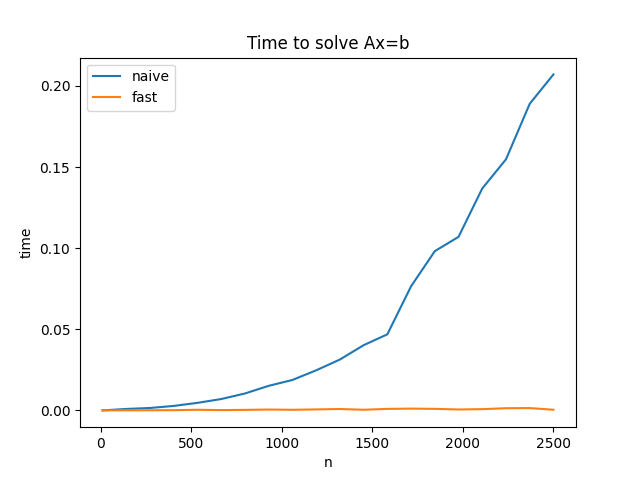
\includegraphics[width=0.5\textwidth]{69d.png}
    \caption{Time of the two methods}
    \label{fig:69d}
\end{figure}
\section*{Exercise A6.15}
\subsection*{(a)}
We have
\begin{align*}
    Q\begin{bmatrix}
        I_n & 0\\
        0 & -I_n
    \end{bmatrix}Q^T&=\frac{1}{2}
    \begin{bmatrix}
        I_n & I_n\\
        J_n & -J_n
    \end{bmatrix}
    \begin{bmatrix}
        I_n & 0\\
        0 & -I_n
    \end{bmatrix}
    \begin{bmatrix}
        I_n & J_n\\
        I_n & -J_n
    \end{bmatrix}\\
    &=\frac{1}{2}
    \begin{bmatrix}
        I_n & I_n\\
        J_n & -J_n
    \end{bmatrix}
    \begin{bmatrix}
        I_n & J_n\\
        -I_n & J_n
    \end{bmatrix}\\
    &=\frac{1}{2}
    \begin{bmatrix}
        0 & 2J_n\\
        2J_n & 0
    \end{bmatrix}\\
    &=\begin{bmatrix}
        0 & J_n\\
        J_n & 0
    \end{bmatrix}
\end{align*}
If a matrix is orthogonal then we have that $Q^TQ=I_{2n}$, therefore we have that
\begin{align*}
    Q^TQ&=\frac{1}{2}\begin{bmatrix}
        I_n & J_n\\
        I_n & -J_n
    \end{bmatrix}
    \begin{bmatrix}
        I_n & I_n\\
        J_n & -J_n
    \end{bmatrix}\\
    &=\frac{1}{2}\begin{bmatrix}
        2I_n & 0\\
        0 & 2I_n
    \end{bmatrix}\\
    &=I_{2n}
\end{align*}
So $Q$ is orthogonal.
\subsection*{(b)}
We have
\begin{align*}
    J_{2n}A&=AJ_{2n}\\
    Q^TJ_{2n}A&=Q^TAJ_{2n}\\
    Q^TJ_{2n}AQ&=Q^TAJ_{2n}Q\\
    Q^TJ_{2n}AQ&=Q^TAQ\begin{bmatrix}
        I_n & 0\\
        0 & -I_n
    \end{bmatrix}Q^TQ\\
    Q^TJ_{2n}AQ\begin{bmatrix}
        I_n & 0\\
        0 & -I_n
    \end{bmatrix}&=Q^TAQ\begin{bmatrix}
        I_n & 0\\
        0 & -I_n
    \end{bmatrix}\begin{bmatrix}
        I_n & 0\\
        0 & -I_n
    \end{bmatrix}\\
    Q^TJ_{2n}AQ\begin{bmatrix}
        I_n & 0\\
        0 & -I_n
    \end{bmatrix}&=Q^TAQ\\
    Q^TAQ&=\begin{bmatrix}
        I_n & 0\\
        0 & -I_n
    \end{bmatrix}Q^TAQ\begin{bmatrix}
        I_n & 0\\
        0 & -I_n
    \end{bmatrix}\\
    Q^TAQ&=\frac{1}{2} \begin{bmatrix}
        I_n & J_n\\
        -I_n & J_n
    \end{bmatrix} A \begin{bmatrix}
        I_n & -I_n\\
        J_n & J_n
    \end{bmatrix}
\end{align*}
Let us express $A$ in terms of n x n submatricies, $B$, $C$, $D$, and $E$. 
We have
$A=\begin{bmatrix}
    B & D\\
    E & C
\end{bmatrix}$, and
\begin{align*}
    J_{2n}A&=AJ_{2n}\\
    \begin{bmatrix}
        0 & J_n\\
        J_n & 0
    \end{bmatrix}
    \begin{bmatrix}
        B & D\\
        E & C
    \end{bmatrix}
    &=\begin{bmatrix}
        B & D\\
        E & C
    \end{bmatrix}
    \begin{bmatrix}
        0 & J_n\\
        J_n & 0
    \end{bmatrix}\\
    \begin{bmatrix}
        J_nE & J_nC\\
        J_nB & J_nD
    \end{bmatrix}&=\begin{bmatrix}
        DJ_n & BJ_n\\
        CJ_n & EJ_n
    \end{bmatrix}
\end{align*}
Therefore we have:
\begin{align*}
    Q^TAQ&=\frac{1}{2} \begin{bmatrix}
        I_n & J_n\\
        -I_n & J_n
    \end{bmatrix} A \begin{bmatrix}
        I_n & -I_n\\
        J_n & J_n
    \end{bmatrix}\\
    &=\frac{1}{2} \begin{bmatrix}
        I_n & J_n\\
        -I_n & J_n
    \end{bmatrix} \begin{bmatrix}
        B & D\\
        E & C
    \end{bmatrix} \begin{bmatrix}
        I_n & -I_n\\
        J_n & J_n
    \end{bmatrix}\\
    &=\frac{1}{2} \begin{bmatrix}
        I_n & J_n\\
        -I_n & J_n
    \end{bmatrix} \begin{bmatrix}
        B+DJ_n & -B+DJ_n\\
        E+CJ_n & -E+CJ_n
    \end{bmatrix}\\
    &=\frac{1}{2} \begin{bmatrix}
        B+DJ_n+J_nE+J_nCJ_n & -B+DJ_n-J_nE+J_nCJ_n\\
        -B-DJ_n+J_nE+J_nCJ_n & B-DJ_n-J_nE+J_nCJ_n
    \end{bmatrix}
\end{align*}
From $J_{2n}A=AJ_{2n}$ we get that $DJ_n-J_nE=0$ and 
$CJ_n-J_nB=0$. Therefore we have that $-B+DJ_n-J_nE+J_nCJ_n=0$
and $-B-DJ_n+J_nE+J_nCJ_n=0$ and thus we get:
$$Q^TAQ=\frac{1}{2} \begin{bmatrix}
        B+DJ_n+J_nE+J_nCJ_n & 0\\
        0 & B-DJ_n-J_nE+J_nCJ_n
    \end{bmatrix}$$
\subsection*{(c)}
Multiplying both sides of $Ax=b$ by $Q^T$ we get:
$$Q^TAQx=Q^Tb$$
Then letting $x=Qy$ we get
$$Q^TAQy=Q^Tb$$
Since $Q^TAQ$ is block diagonal, this is just solving
two n x n systems of equations. which will take $2\cdot\frac{2}{3}n^3$
operations. Since multiplying $b$ by $Q^T$ takes $2n^2$ operations,
and multiplying $y$ by $Q$ takes $2n^2$ operations, we have that
the leading term of our imporoved solution is $\frac{4}{3}n^3$ So
we have been able to reduce the number of flops by a factor if $4$.
\section*{Exercise A6.16}
We have that 
$$A_{ij}=\sum_{k=1}^n Q_{ik}R_{kj}$$
Since $R$ is upper triangular we have that 
$$A_{ij}=\sum_{k=1}^j Q_{ik}R_{kj}$$
Since we have that $A_{ij}=0$ for $i>j+1$, and since $R_{kj}$
is not necessarily $0$ for $k\leq j$ then we have that
$Q_{ik}=0$ for $k\leq j<i-1$. Therefore we have that
$Q_{ij}=0$ for $i>j+1$.  

\section*{Exercise A7.5}
We first LU factorize $A$, which will cost us $\frac{2}{3}n^3$ flops. 
Then we solve for $x'=A^{-1}b$, which will cost us $2n^2$ flops, then with this we can
solve for $x''=A^{-2}b=A^{-1}x'$, which will cost us $2n^2$ flops.
Then once again, solving for $x'''=A^{-3}b=A^{-1}x''$, which will cost us $2n^2$ flops.
then sum up $b$ and $x'$, $x''$, $x'''$ to get $x$, which will cost us 
$3n$ flops. So in total we will take $\boxed{\frac{2}{3}n^3+6n^2+3n}$ flops.
\section*{Exercise A7.10}
First we LU factorize $A$, which will cost us $\frac{2}{3}n^3$ flops. 
Then we solve for $x=A^{-1}b$, which will cost us $2n^2$ flops, and we solve
for $x_u=A^{-1}u$, which will cost us $2n^2$ flops, then we have
$$y=(A+uv^T)^{-1}b=x-\frac{1}{1+v^Tx_u}x_uv^Tx$$
Then we calculate $v^Tx_u$, which will cost us $2n-1$ flops and 
$v^Tx$ which will likewise cost $2n-1$ flops. Then we have
$$y=(A+uv^T)^{-1}b=x-\frac{v^Tx}{1+v^Tx_u}x_u$$
Solving for x consists of first of all finding $\frac{x_uv^T}{1+v^Tx_u}$ given 
$v^Tx_u$ and $v^Tx$, which will cost $2$ flops, and then we multiply that value 
to every value in $x_u$, which will cost us $n$ flops, and then subtracting
the resulting vector from $x$ will once again cost us $n$ flops, 
thus we have that the total flops needed would be:
$$\frac{2}{3}n^3+4n^2+4n+2n=\boxed{\frac{2}{3}n^3+4n^2+6n}$$




  


\end{document}